\documentclass{article}
\usepackage[utf8]{inputenc}
\usepackage[legalpaper, portrait, margin=1in]{geometry}
\usepackage[T1]{fontenc}
\usepackage{multirow}
\usepackage{tabu}
\usepackage{graphicx}
\usepackage{subcaption}
\usepackage{amsmath}
\usepackage{media9}

\newcommand{\etal}{\textit{et al.}}
\newcommand{\norm}[1]{\left\lVert#1\right\rVert}

\title{Towards Point Cloud Rotation Invariance using Point Pair Features}
\author{Qiao Gu \\
  Andrew ID: qiaog
  \and
  Yanjia Duan \\
  Andrew ID: yanjiad
  }
% \date{March 2021}
\date{}

\begin{document}

\maketitle

\includemedia[
  width=0.6\linewidth,height=0.45\linewidth,
  activate=pageopen,
  flashvars={
    modestbranding=1 % no YT logo in control bar
   &autohide=1       % controlbar autohide
   &showinfo=0       % no title and other info before start
  }
]{}{https://youtu.be/Wkdv5R0nSGg}

\section{Introduction}

Deep learning on 3D point cloud has been widely studied by the computer vision community over the past few years \cite{Qi2017pointnet, qi2017pointnet2, Wang2019-dgcnn, Li2018-PointCNN}. 
However, a recent benchmark \cite{taghanaki2020robustpointset} demonstrates that most of these network structures are not rotation invariant and their performance drops dramatically if no rotation augmentation is applied during training while the point cloud is randomly rotated at test time. 
We believe that this is because in most deep neural networks for point cloud, the input is Cartesian coordinates of each point. PointNet \cite{Qi2017pointnet}, as one of the most basic architectures, projects the point coordinates into a high-dimensional space using per-point MLP, then uses a max-pooling layer to extract occupancy in the high-dimensional space, which maps back to complex geometric surfaces in the original space. This essentially gives a description of the shape of the point cloud, which could be used in point cloud classification and segmentation tasks.
However, taking raw coordinates as input requires the input point cloud to be aligned with a ``canonical'' pose, and this necessitates the input 6-DoF transformation proposed in~\cite{Qi2017pointnet}. 

Therefore, in the project, we explore the usage of Point Pair Features (PPF), a rotation-invariant representation that has been widely used for 6D pose estimation and the point cloud registration task in the context of deep neural networks. We specifically focus on improving the rotation robustness of these networks by incorporating the special invariant property of PPF. 
We adapt the widely-used PointNet \cite{Qi2017pointnet}, PointNet\texttt{++} \cite{qi2017pointnet2} and Dynamic Graph CNN (DGCNN) \cite{Wang2019-dgcnn} structures and change their input to per-point PPF featurizaion instead of pure 3D point coordinates. 
We design several simple sampling strategies to select the reference point and convert each point in the point cloud to the 4-dimensional PPF vector. We demonstrate that incorporating PPF features can greatly improve the rotation robustness in the absence of training-time rotation augmentation. 
However, when applying training time augmentation used in \cite{qi2017pointnet2}, we found that PPF featurization leads to unstable performance. We hypothesize that this is because the straightforward sampling strategies we adopt are not robust to point cloud perturbation.
Moreover, taking the inspiration from PointNet\texttt{++} \cite{qi2017pointnet2}, we incorporate the PPF featurization in the first point set abstraction layer and use sampled group centers as reference points, which improved the test time classification accuracy by 1.84\%.

% This is because PointNet, as one of the earliest explorations on point cloud learning, has a simple network structure and is designed to be invariant to the order of points. 
% Then taking the inspiration from PointNet++ \cite{qi2017pointnet2}, we will design a hierarchical learning framework by stacking multiple stages. Note that one key insight of PPF is computing relative relationship between points as distances and relative angles. We would also explore the idea of computing relative relations between point features in the latent space (e.g. abstract point features in the intermediate layers of PointNet++). 

% For experiments, we think that the point cloud classification and segmentation tasks should be a good starting point, which we expect to be simpler and less tricky than learning local descriptors that require a contrastive learning framework. Following the most popular practice in the literature, we will use the ShapeNet \cite{Chang2015-ShapeNet} and ModelNet \cite{Wu2015-3dshapenet} datasets. Also RobustPointSet \cite{taghanaki2020robustpointset} has defined a good benchmarking protocol to evaluate different aspect of the robustness and invariance on point cloud learning, which we will also follow to evaluate our method. 

\section{Related Work}

\subsection{3D Perception}

3D perception has been extensively studied by the deep learning community, and point cloud is one of the most prevalent data formats for 3D representation. Numerous network architectures~\cite{Qi2017pointnet, qi2017pointnet2, Wang2019-dgcnn, Li2018-PointCNN, Wu2019-pointconv, Liu2019-densepoint} have been proposed over the past few years to learn feature representations useful for the down-streaming tasks (i.e. classification, segmentation, generation, etc.). While these methods tackled the challenges brought by point cloud irregularity, unstructuredness, and unorderedness, a recent work~\cite{taghanaki2020robustpointset} showed that they are not robust to different types of point cloud perturbation (noise, translation, occlusion, etc) and will fail significantly when test-time rotation perturbation is applied. Most methods only achieved around 10\% classification accuracy on rotated ModelNet~\cite{Wu2015-3dshapenet} testing set. 
SPHnet \cite{Poulenard2019-sphnet} and PRIN \cite{You2021-prin} show their invariance to rotated point clouds by specially-designed rotation-invariant local features and network structures, but their basic performance on point cloud classification is reported to be much lower than other networks. 


\subsection{Point Pair Features}

Point Pair Feature (PPF), first proposed by Drost.~\etal~\cite{Drost2010-ppf}, is a four-dimensional feature describing the relative relationship between two points in the same point cloud. Determined by its design, it is completely invariant to any 6D transformation, including rotation and translation. Even without any deep learning components, PPF has shown its great power in 6D pose estimation~\cite{Eunyoung_Kim2011-3dobject, Birdal2015-ppfbased, Hinterstoisser2016-goingfurther, Kiforenko2018-ppfeval}, and one variant of it \cite{Vidal2018-rh} is still among the state-of-the-art methods in BOP Challenge \cite{Hodan2018-bop}. Some recent works \cite{Deng2018-PPFNet, Deng2018-PPFFoldNet} exploit the power of PPF in designing 3D local descriptors and show great performance in point cloud registration. But the power of PPF is still relatively under-explored in the deep learning context, and to our best knowledge, no work has integrated PPF into deep neural networks for point cloud classification or segmentation. 

\section{Method}

We designed two strategies for PPF featurization, which are (1) input-level featurization, (2) anchor point-based featurization. The input-level featurization is performed on PointNet, PointNet\texttt{++} and DGCNN. Anchor point-based featurization is performed on PointNet\texttt{++}. We will explain the concept of point pair features in subsection \ref{section:PPF}, input-level featurization in \ref{section:PPF_inp} and anchor point-based featurization in \ref{section:PPF_anchor}.

\subsection{Background Point Pair Features}
\label{section:PPF}

Point Pair Features (PPF), introduced in~\cite{Drost2010-ppf}, extracts four numbers from a pair of points and their surface normal vectors, which describes the relative geometric relationship between the two points. Given two point clouds, if we can find one PPF from each point cloud respectively, we can estimate a 6 degree-of-freedom (DoF) rigid body transformation by aligning these points and normal vectors. Object pose estimation or point cloud registration can therefore be achieved by iterating over all matching pair of PPFs and conducting a Hough voting algorithm. This process can be followed by a pose clustering and refinement step to further improve the accuracy. In this project, we just take the basic PPF featurization and will briefly introduce it below. For a comprehensive introduction, please refer to~\cite{Drost2010-ppf, Vidal2018-rh}. 

\begin{figure}[t]
    \centering
    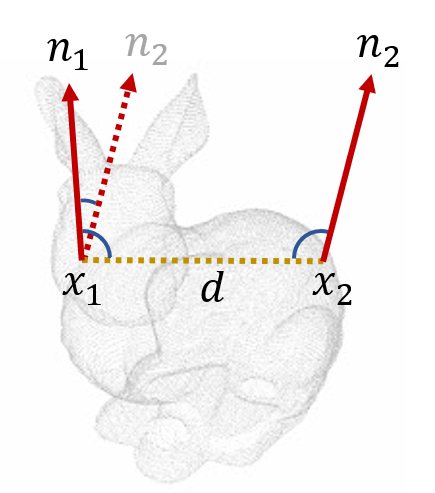
\includegraphics[width=0.25\linewidth]{images/ppf.png}
    \caption{Illustration of Point Pair Feature on a point cloud. }
    \label{fig:ppf_illu}
\end{figure}

As shown in Fig.~\ref{fig:ppf_illu}, given a point cloud, we first sample $x_1$ as the reference point and then sample $x_2$ as the second point. We denote the surface normal vectors at these two points as $n_1$ and $n_2$, and the distance vector from $x_1$ to $x_2$ is $d=x_2-x_1$. Point Pair Feature $\psi_{12}$ contains 4 numbers, including a distance vector and three angles. And they are defined as 
\begin{align}
    \psi_{12} = (\norm{d}_2, \; \angle (n_1, d), \; \angle(n_2, d), \; \angle (n_1, n_2)),
\end{align}
where $\norm{\cdot}_2$ denotes $L$-2 vector norm and $\angle(\cdot, \cdot)$ computes the angle between two vectors. For numerical stability, we compute the angle as following \cite{Birdal2015-ppfbased}
\begin{align}
    \angle(v_1, v_2) = \arctan(\norm{v_1 \times v_2}, v_1\cdot v_2).
\end{align}

Apparently, a point pair feature describes the relative relationship between two points and is agnostic to the actual position or orientation of the point cloud. Therefore, PPF is invariant to any rigid body transformation as long as the point cloud shape does not change.  


\subsection{Global PPF Featurization}
\label{section:PPF_inp}

\begin{figure}[hbt!]
\centering
    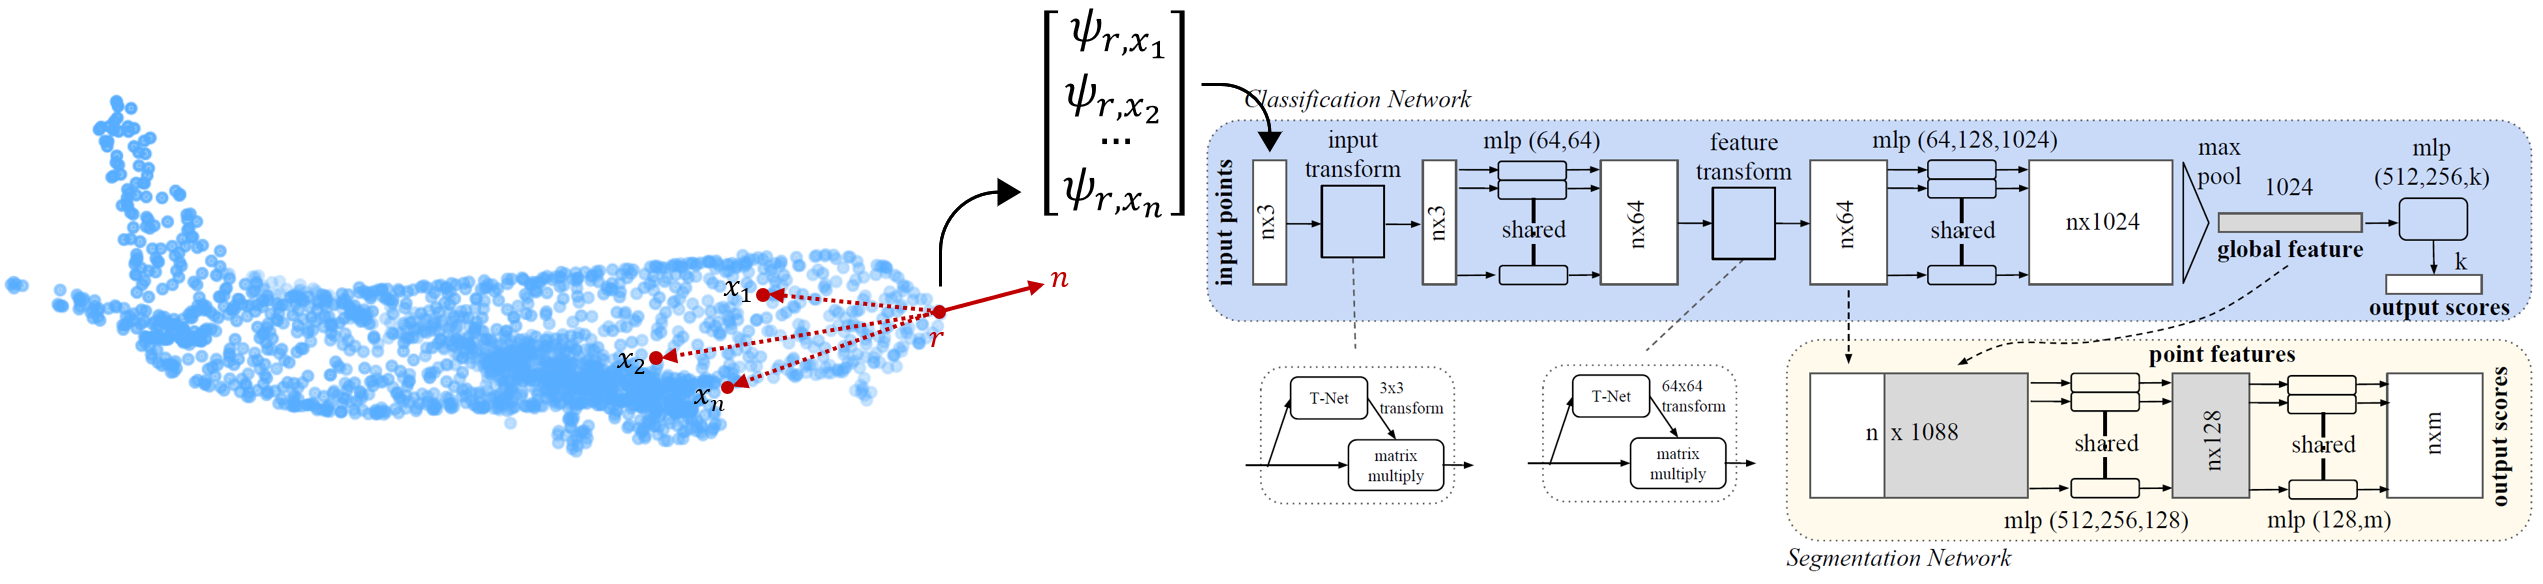
\includegraphics[width=.9\linewidth]{images/pn_input.png}
    \caption{PPF featurization as input to PointNet.}
\label{fig:pn_input}
\end{figure}

We first tried a simple method of converting input point clouds to PPF features. We sample a single point $r$ as the reference point and then compute the 4D PPFs for all other points with respect to $r$. As shown in Fig.~\ref{fig:pn_input}, the mapping from point cloud to PPFs can be expressed as 
\begin{align}
    M_1 : 
    \begin{bmatrix}
    r \\ x_1 \\ x_2 \\ \cdots \\ x_n
    \end{bmatrix}
    \rightarrow
    \begin{bmatrix}
    \psi_{r,x_1} \\ \psi_{r,x_2} \\ \cdots \\ \psi_{r,x_n}.
    \end{bmatrix}
\end{align}

And we also designed different strategies for sampling $r$:
\begin{itemize}
    \item \textit{PPF (Random)}: we sample a random point in the point cloud as $r$. 
    \item \textit{PPF (Center)}: we first compute the mean position of the point cloud $x_c=\sum_{i=1}^n x_I / n$ and then choose the point closest to $x_c$ as $r$, which means $x_c = \arg\min_{x_i} \norm{x_c-x_i}_2$. 
    \item \textit{PPF (Farthest)}: We use the point that is furthest from $x_c$ as $r$, which means $x_c = \arg\max_{x_i} \norm{x_c-x_i}_2$. 
\end{itemize}

This method input featurization is agnostic to the network architecture and can be used for any point cloud network. 

\subsection{Local PPF Featurization Based on Anchors}
\label{section:PPF_anchor}

\begin{figure}[hbt!]
\centering
    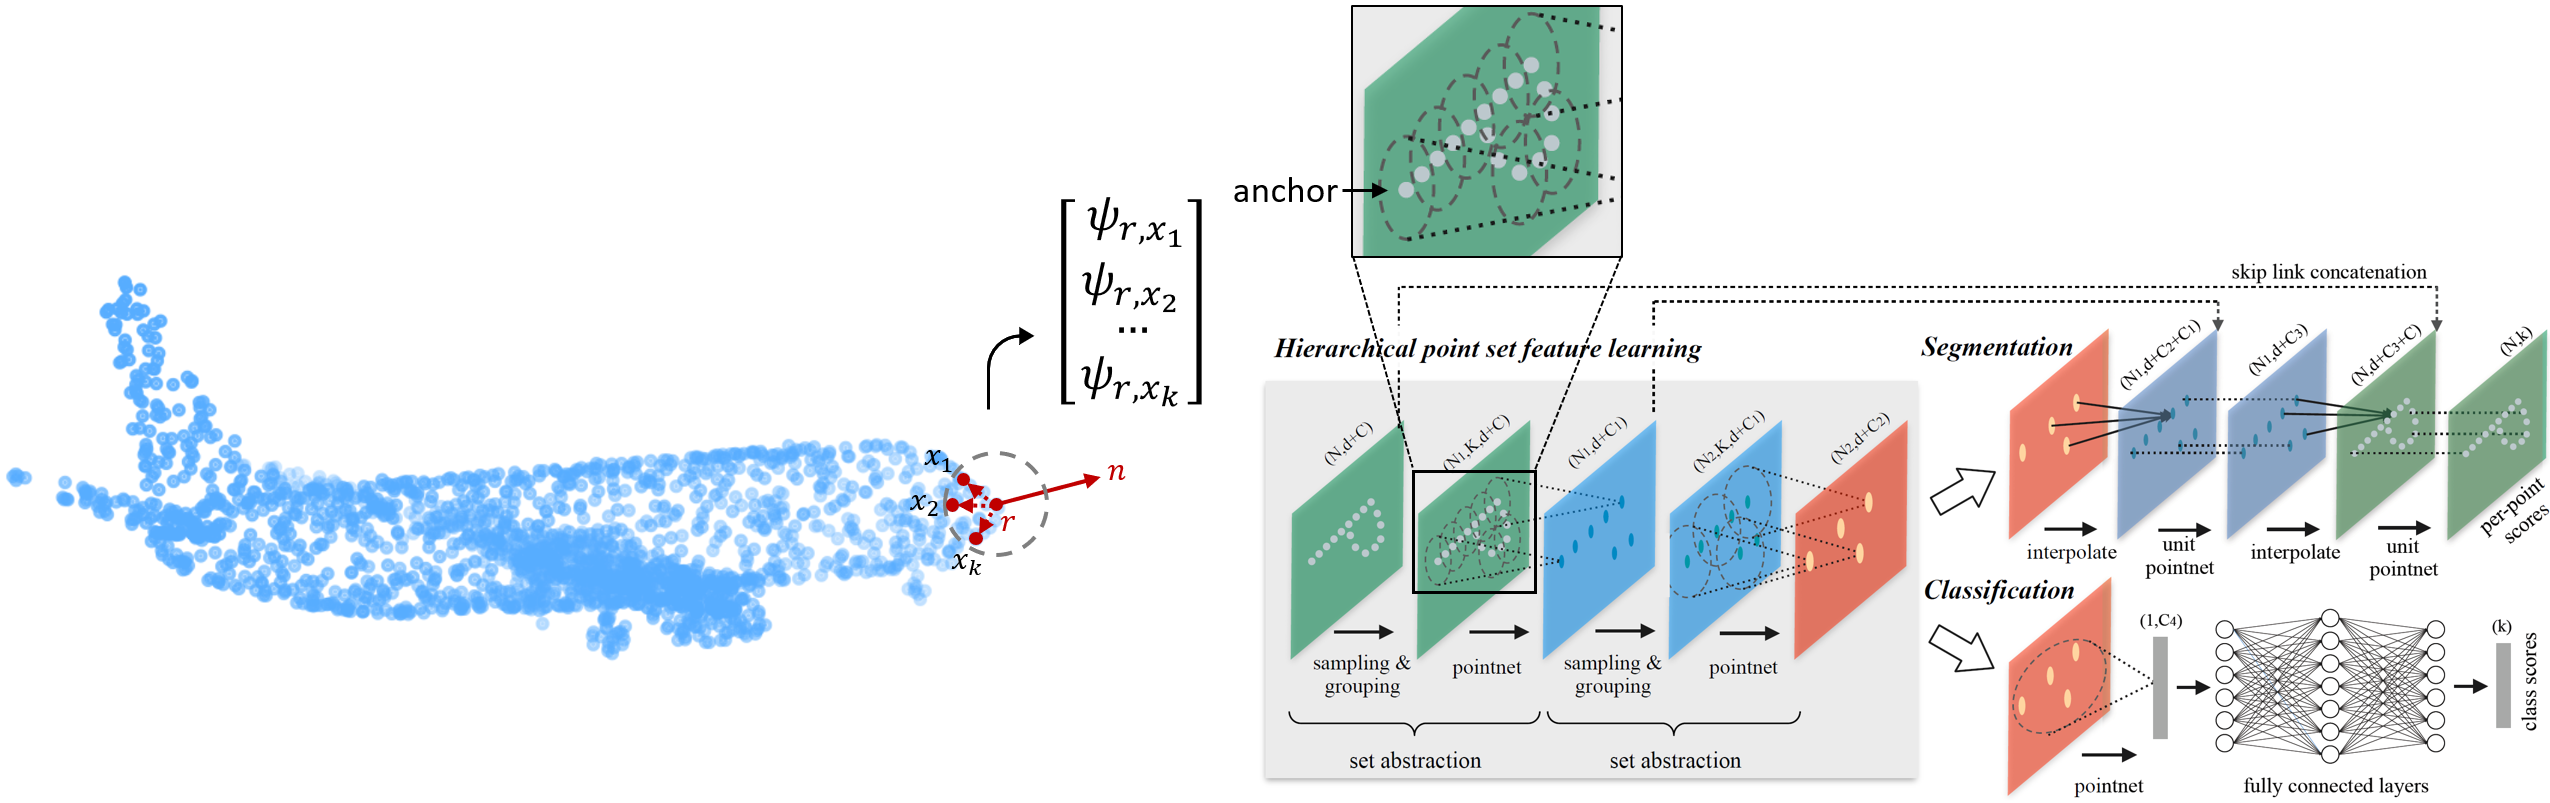
\includegraphics[width=.9\linewidth]{images/pn2_input.png}
    \caption{PPF featurization based on anchor point in the first Set Abstraction layer.}
\label{fig:pn2_input}
\end{figure}

We also incorporated the PPF featurization into the hierarchical architecture of PointNet\texttt{++}~\cite{qi2017pointnet2}. Specifically, in the Set Abstraction layers, PointNet\texttt{++} first samples some anchors, then for each anchor, find their K nearest neighbors to form a small point cloud. Each small point cloud runs through a PointNet. In the first Set Abstraction layer, we treat the sampled anchor of each group as the reference point $r$ and compute PPF $\psi_{r, x_i}$ ($i\in\{1,..., k\}$) for every point $x_i$ in the small group. As shown in Fig.~\ref{fig:pn2_input}, the computed PPFs are then fed into PointNet. We call this sampling strategy \textit{PPF (anchor)}.

\section{Experiment}

\subsection{Dataset}

To evaluate our design of PPF featurization, we use the ModelNet40~\cite{Wu2015-3dshapenet} dataset. ModelNet40 contains 12,308 CAD models of 40 different categories, which are split into a training set of 9,840 objects and a testing set of 2,468 objects. We sub-sampled the CAD models and get 2,048 points for each point cloud, together with their surface normal vectors. We adopt the point cloud classification task, where the network is going to output a 40-dimensional probability distribution, one for each category. In the experiments below, we report the classification accuracy averaged over 40 categories. 

\begin{table}[hbt!]
    \centering
    \begin{tabular}{ll|c|cc}\hline\hline
         \multicolumn{2}{c|}{\multirow{2}{*}{Architecture}} & Training w/o Augmentation & \multicolumn{2}{c}{Training w/ Augmentation} \\\cline{3-5}
         & & \texttt{Rotated} & \texttt{Original} & \texttt{Rotated} \\\hline
         PointNet \cite{Qi2017pointnet} & \multicolumn{1}{|l|}{$Spatial$} & 21.68 & - & - \\
         & \multicolumn{1}{|l|}{$Spatial+Normal$} & 22.56 & 81.50 & 77.80 \\
         & \multicolumn{1}{|l|}{$PPF\ (Random)$} & 64.30 & - & - \\
         & \multicolumn{1}{|l|}{$PPF\ (Center)$} & \textbf{73.79} & 26.07 & 25.35 \\
         & \multicolumn{1}{|l|}{$PPF\ (Farthest)$} & 60.82 & - & - \\\hline
         PointNet\texttt{++ \cite{qi2017pointnet2}} & \multicolumn{1}{|l|}{$Spatial\texttt{++}Normal$} & 28.85 & \textbf{87.01} & 84.30 \\
         & \multicolumn{1}{|l|}{$PPF\ (Center)$} & 53.24 & - & - \\
         & \multicolumn{1}{|l|}{$PPF\ (Anchor)$} & \textbf{69.69} & 86.28 & \textbf{86.14}  \\\hline
         DGCNN \cite{Wang2019-dgcnn} & \multicolumn{1}{|l|}{$Spatial$} & 26.68 & - & - \\
         & \multicolumn{1}{|l|}{$Spatial\texttt{+}Normal$} & 29.96 & 86.80 & 84.22 \\
         & \multicolumn{1}{|l|}{$PPF\ (Random)$} & 73.08 & - & - \\
         & \multicolumn{1}{|l|}{$PPF\ (Center)$} & \textbf{77.94} & 45.51 & 46.00 \\
         & \multicolumn{1}{|l|}{$PPF\ (Farthest)$} & 72.60 & - & - \\\hline\hline
    \end{tabular}
    \caption{Testing class accuracy on different networks, PPF sampling strategies and training augmentation. The \texttt{Training w/o Augmentation} column shows the result of training on different PPF sampling strategies. The \texttt{Train w/ Augmentation} column shows the result of training on the augmented training point clouds and testing with \texttt{Original} and \texttt{Rotation} test sets.}
    \label{tab:my_label}
\end{table}

\subsection{PPF Sampling Strategies}

We trained different PPF sampling strategies on PointNet, PointNet\texttt{++} and DGCNN on ModelNet40 dataset. 
To study whether the trained network can learn rotation-invariant representation, we follow the evaluation protocol proposed in~\cite{taghanaki2020robustpointset}, and we first perform the experiments where the training data augmentation is disabled, and thus all training point clouds are from the original ModelNet40 (\textit{Training Original}). 
For baseline performance, we separately trained the vanilla networks with only spatial coordinates (\textit{Spatial}) and with spatial coordinates and surface normal vectors (\textit{Spatial + Normal}).
And for the proposed PPF featurization, we train and test using different reference point sampling strategies, including \textit{PPF (Random)}, \textit{PPF (Center)}, and \textit{PPF (Farthest)}. 
For PointNet\texttt{++}, we also trained it on the \textit{PPF (Anchor)} method described in Sec.~\ref{section:PPF_anchor}. 

The results show that in the absence of training data augmentation, networks with \textit{Spatial} and \textit{Spatial + Normal} overfit to the training set and don’t generalize to the rotated point cloud. 
Applying PPF significantly boosts the validation accuracy by 30$\sim$40\%. \textit{PPF (Center)} performs the best on PointNet and DGCNN, with 73.79\% and 77.94\% test-time classification accuracy respectively. \textit{PPF (Anchor)} performs the best on PointNet\texttt{++}, with 69.69\% test-time classification accuracy.

\begin{figure}[ht!]
    \centering
    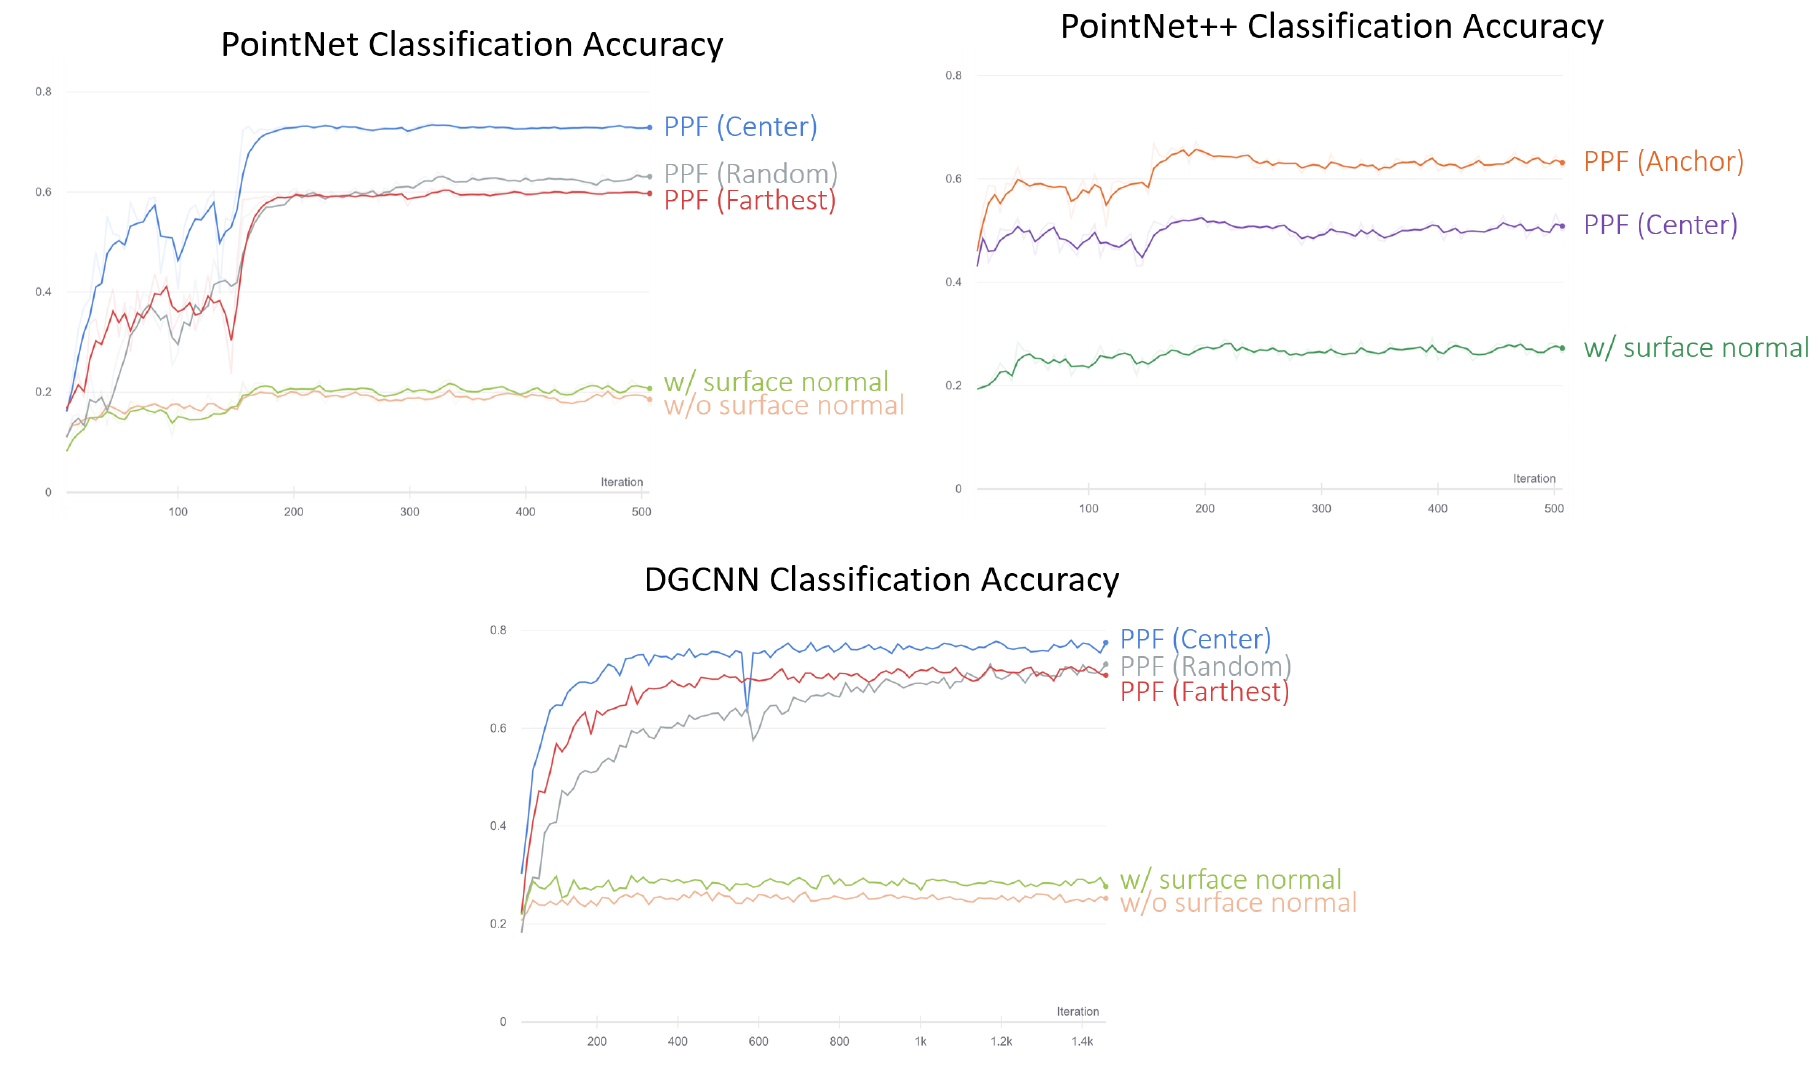
\includegraphics[width=\textwidth]{images/ppf_combined.png}
    % \begin{subfigure}[b]{0.49\textwidth}
    %     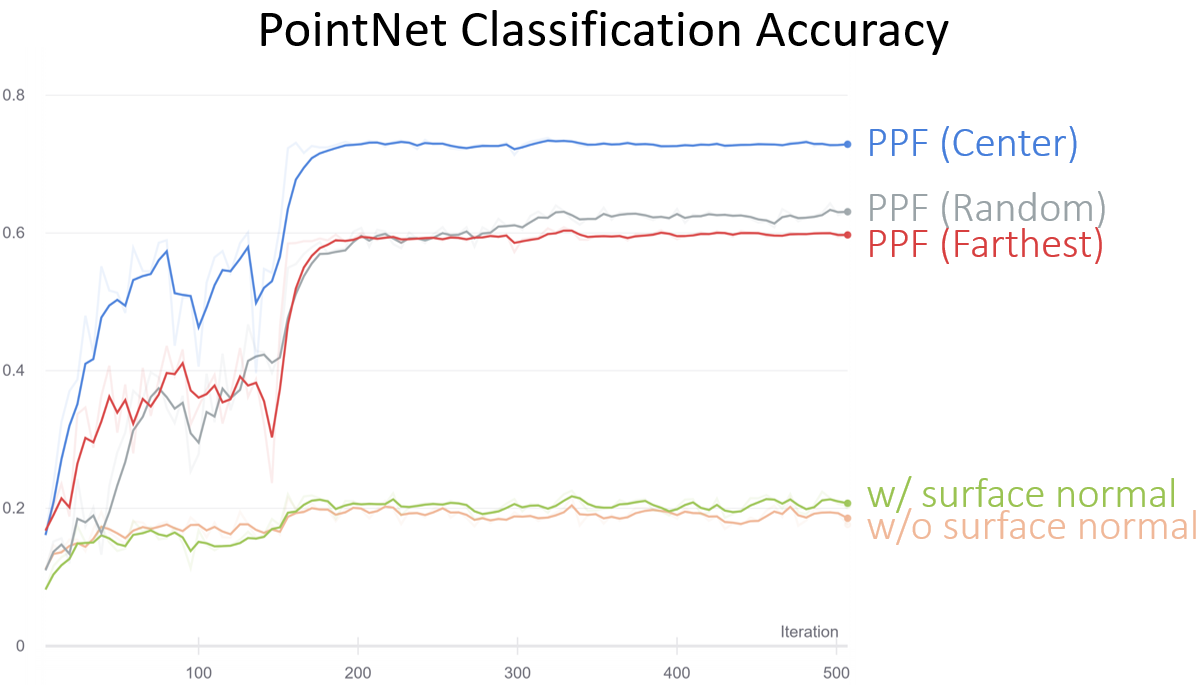
\includegraphics[width=\textwidth]{images/pn_ppf.png}
    % \end{subfigure}
    % \hfill
    % \begin{subfigure}[b]{0.49\textwidth}
    %     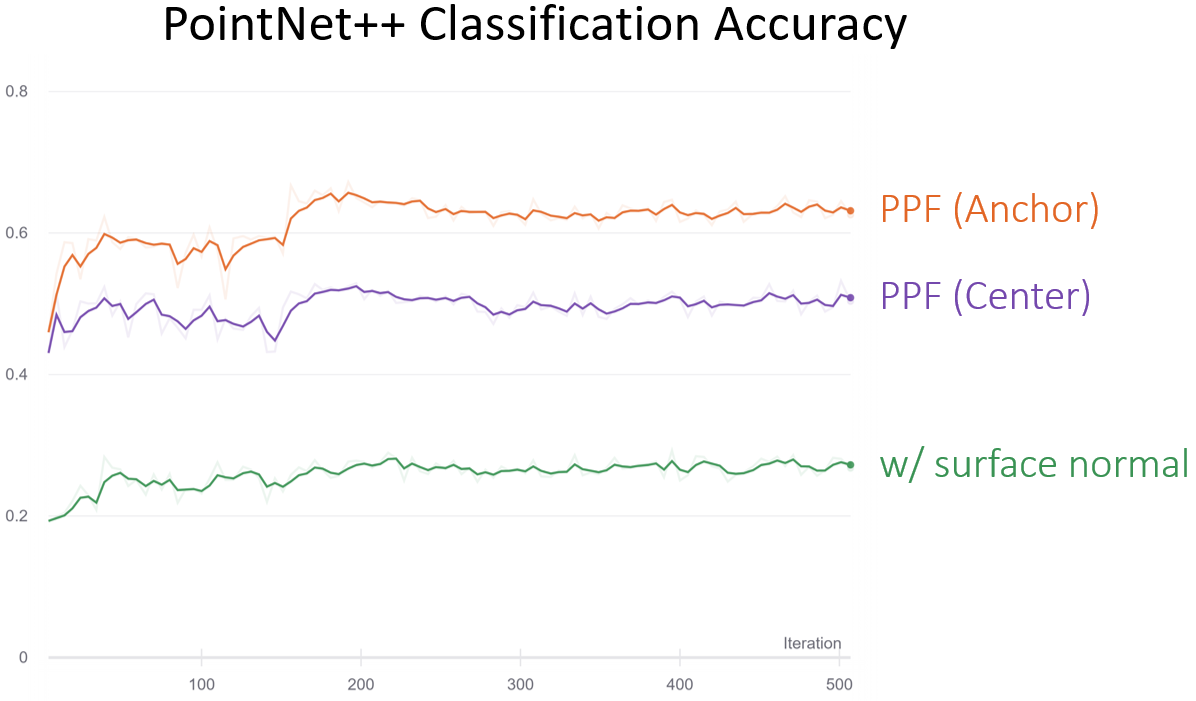
\includegraphics[width=\textwidth]{images/pn2_ppf.png}
    % \end{subfigure}
    % \begin{subfigure}[b]{0.49\textwidth}
    %     \vspace{1em}
    %     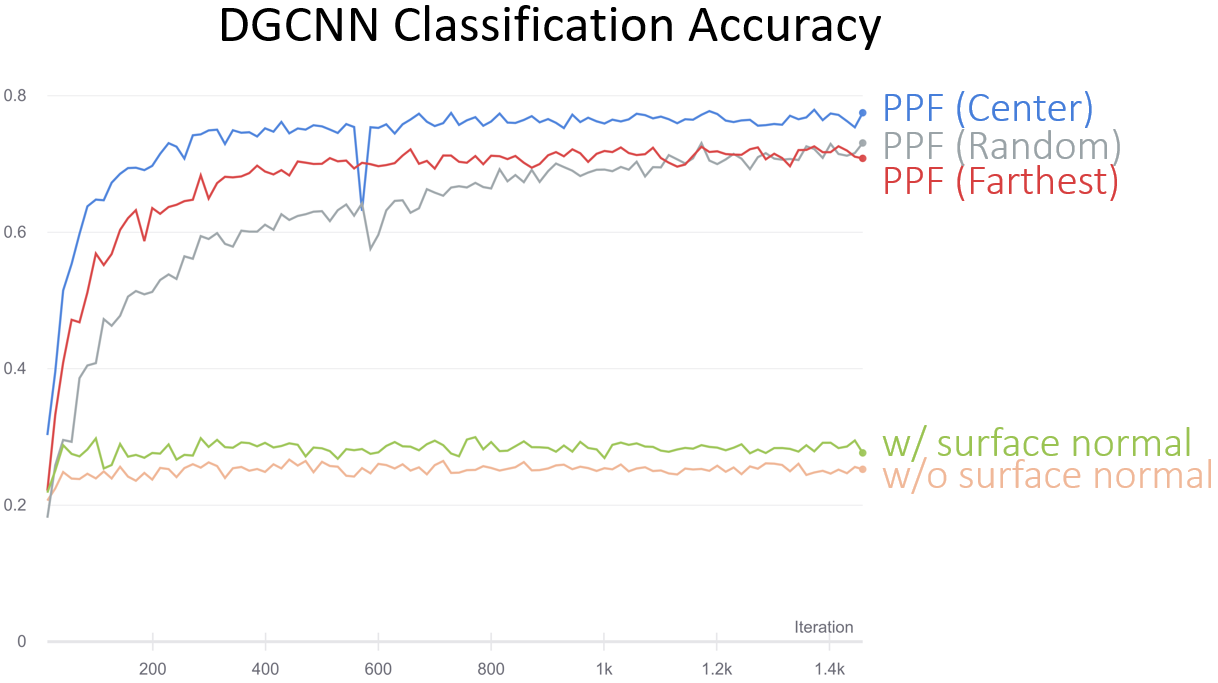
\includegraphics[width=\textwidth]{images/dgcnn_ppf.png}
    % \end{subfigure}
\caption{Classification accuracy on ModelNet40 testing set on different point cloud network using different input featurizations. Note that training augmentation is not used in these experiments. }
\end{figure}

\subsection{Training Augmentation}

% \quad\ We explored the influence of training data augmentation on PPF
However, in the training setup adopted by most point cloud networks, extensive augmentation on point clouds is performed and the trained networks can obtain rotation robustness to some extent. 
Therefore, we also perform experiments following the training data augmentation used in~\cite{qi2017pointnet2}, where the point clouds are randomly rotated, scaled, translated, and jittered. We call this training setup \textit{Training w/ Augmentation} in Table.~\ref{tab:my_label}. And we tested the trained networks on the testing point clouds with and without random rotation perturbation (\textit{Original} and \textit{Rotation})

We can see from the results that using \textit{Spatial+Normal} as input does lead to a performance drop when tested on \textit{Rotated} point clouds, compared to the \textit{Original} ones. 
However, PPF featurization with a single reference for the whole point cloud (\textit{PPF (Center)}) significantly harms the testing accuracy when the training data is augmented. We hypothesize that this is because we sample a single reference point for the whole point cloud, and training data augmentation will constantly change the reference point, which confuses the network learning. 

We tried similarly for PointNet++, except that we use \textit{PPF (anchor)} sampling strategy rather than \textit{PPF (center)}. We can see that applying \textit{PPF (anchor)} on the rotated validation set improves the performance compared to not using it. We think that in the original PointNet++, the difference of spatial coordinates is taken within each group, and using PPF featurization in the local region leads to better test-time rotational robustness. 

\begin{figure}[ht!]
    \centering
    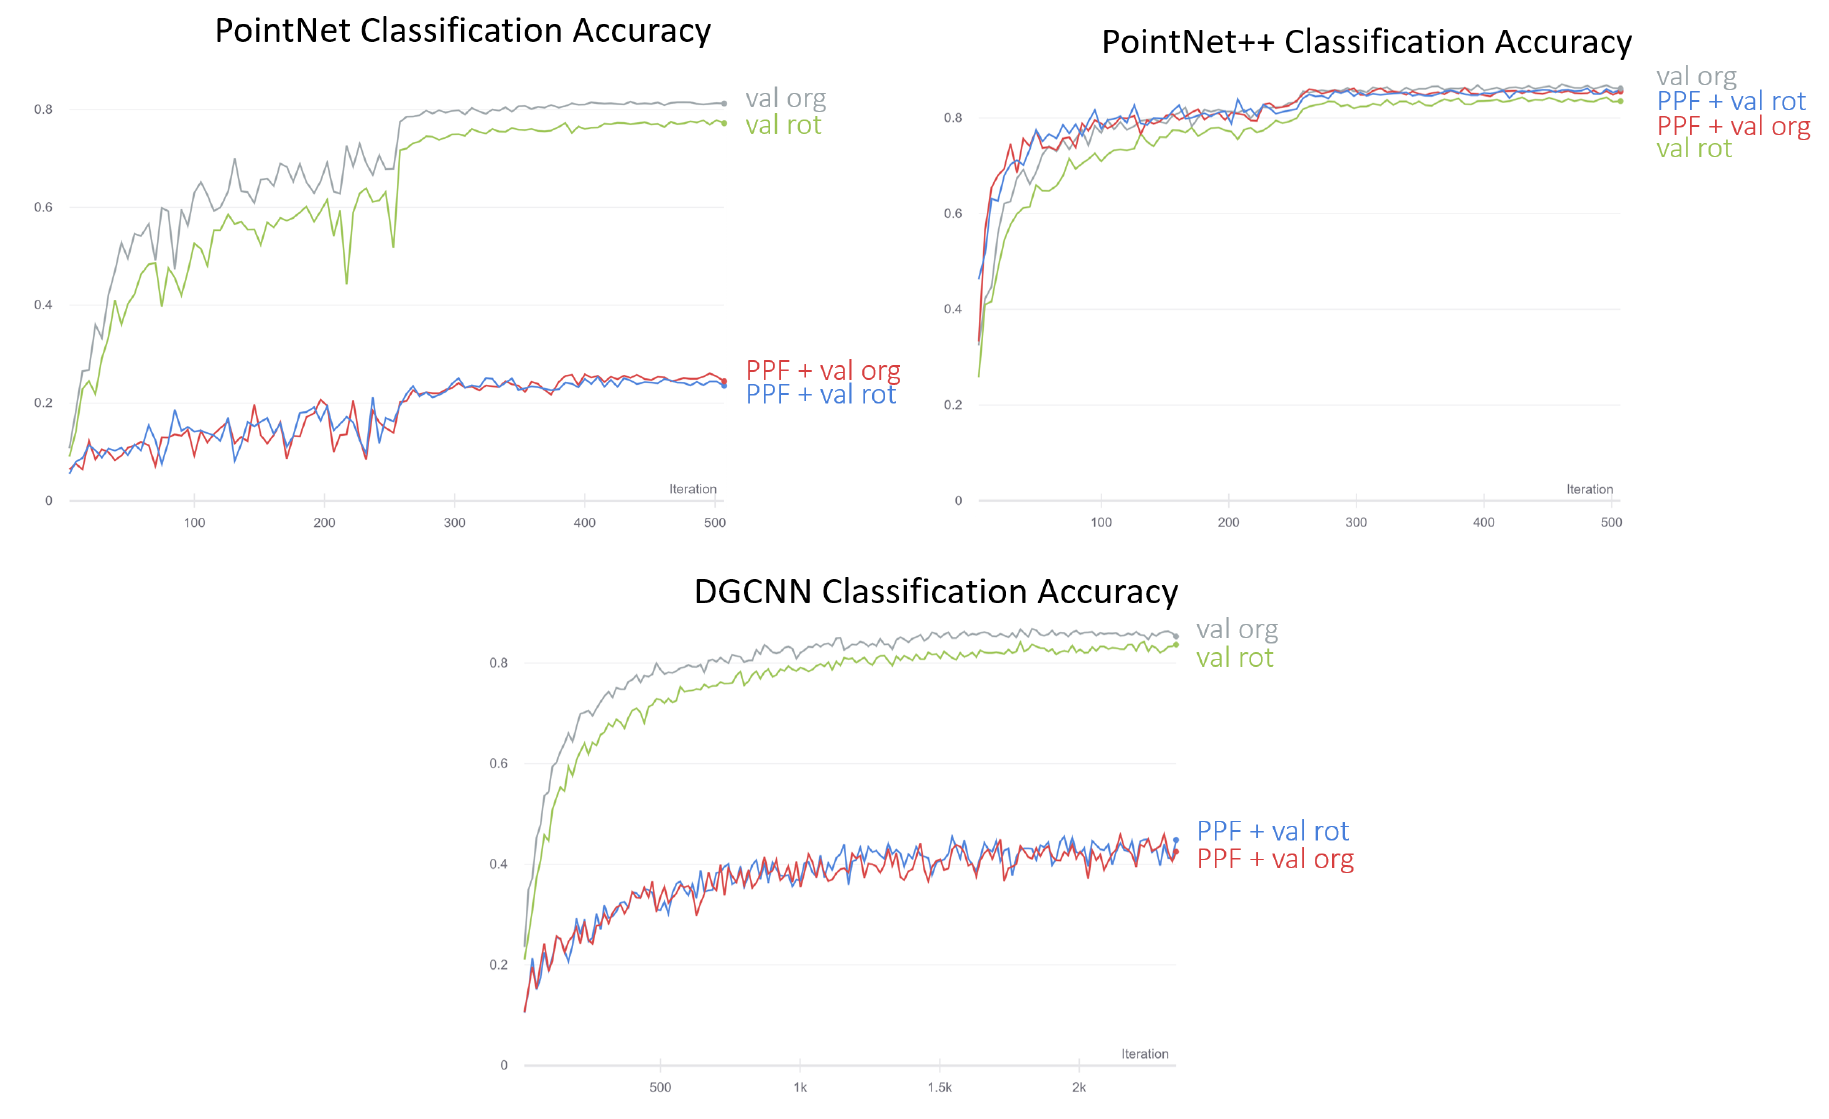
\includegraphics[width=\textwidth]{images/aug_combined.png}
    % \begin{subfigure}[b]{0.49\textwidth}
    %     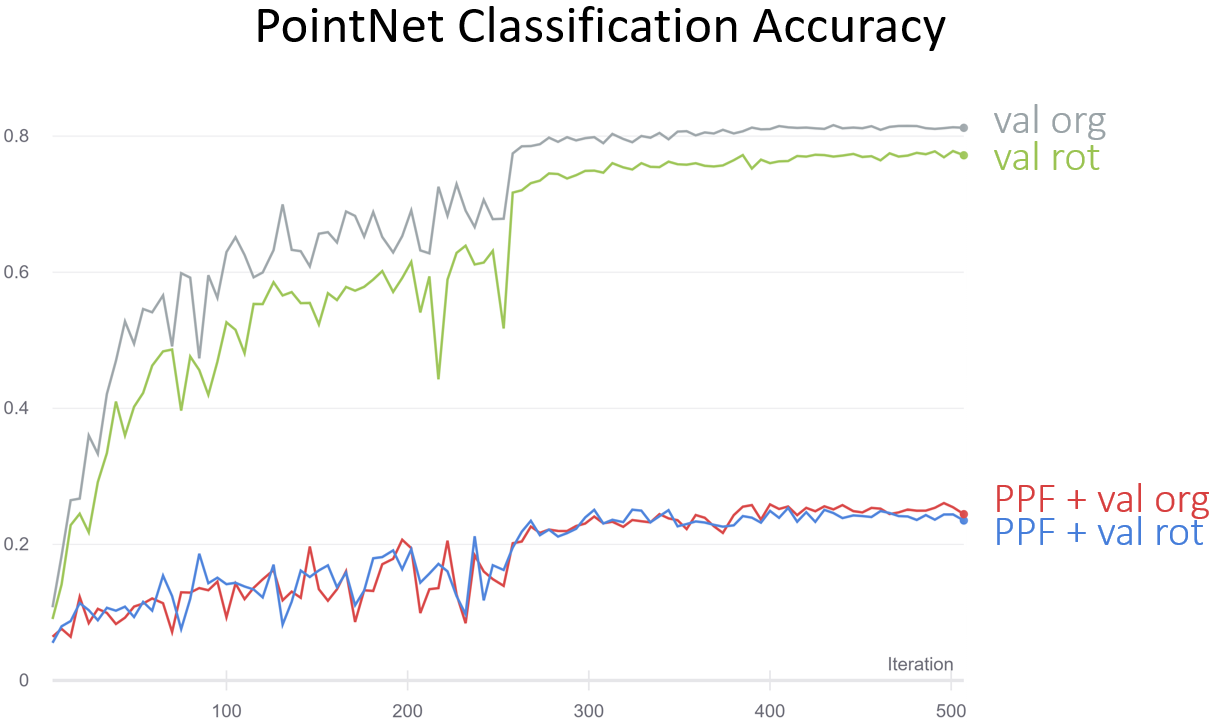
\includegraphics[width=\textwidth]{images/pn_aug.png}
    % \end{subfigure}
    % \hfill
    % \begin{subfigure}[b]{0.49\textwidth}
    %     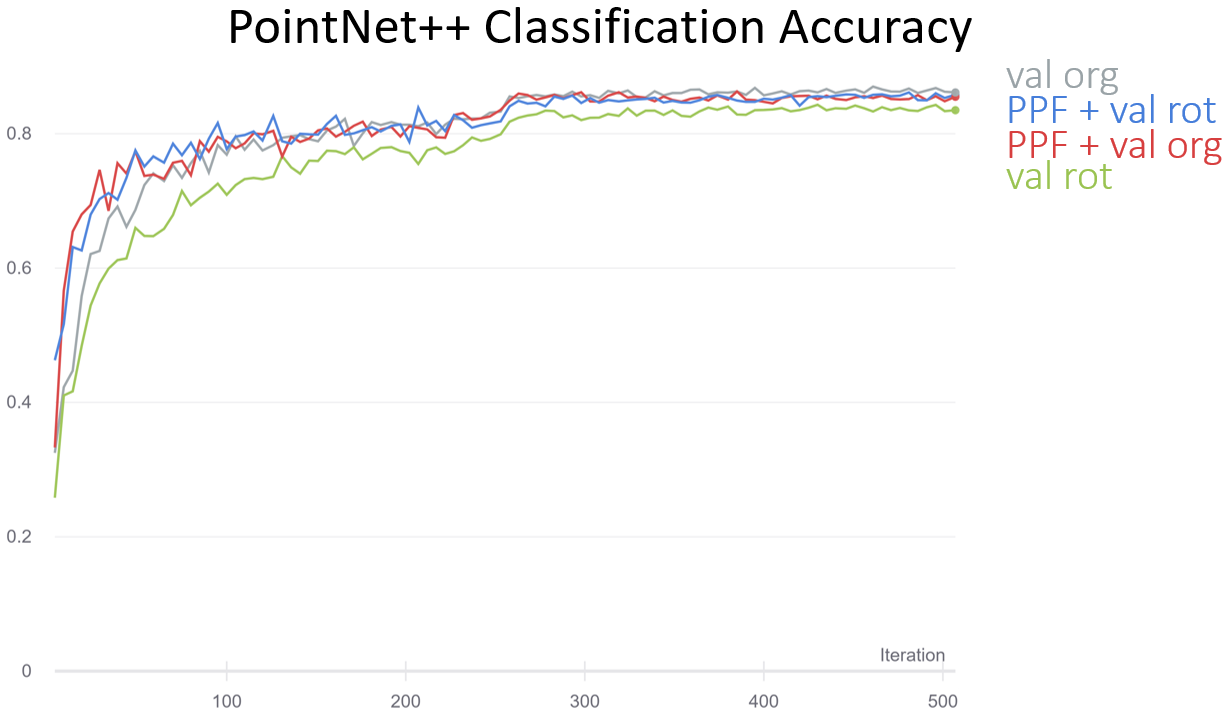
\includegraphics[width=\textwidth]{images/pn2_aug.png}
    % \end{subfigure}
    % \begin{subfigure}[b]{0.49\textwidth}
    %     \vspace{1em}
    %     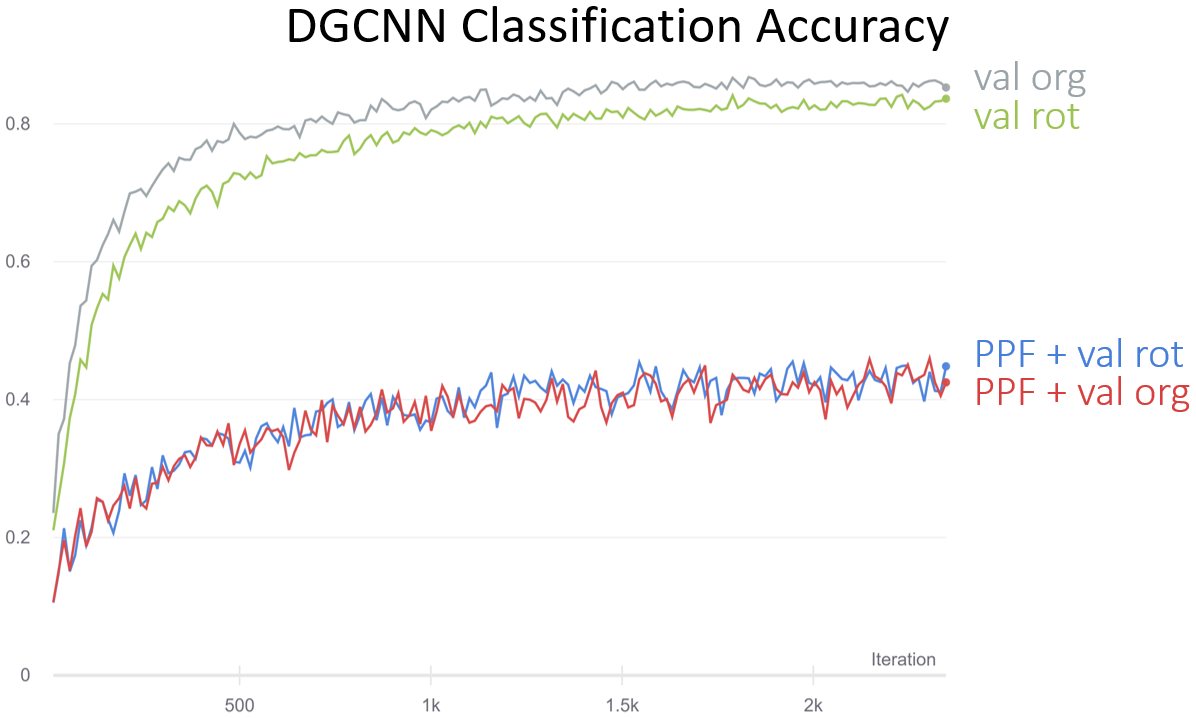
\includegraphics[width=\textwidth]{images/dgcnn_aug.png}
    % \end{subfigure}
\caption{Classification accuracy on ModelNet40 testing set on different point cloud network using different input featurizations. Note that training augmentation used in these experiments.}
\end{figure}

\section{Conclusion and Future Work}

In conclusion, we propose to incorporate PPF featurization into recent deep learning architectures on 3D point clouds. We design and test different strategies of sampling the reference points. The results show that PPF featurization can improve rotational robustness in the absence of training point cloud augmentation. However, sampling a single reference point globally harms the performance when training with augmentation. We also propose to convert a local point cloud to PPFs in the sampling and grouping step in PointNet++, and we find that it improves the rotational robustness in PointNet++. For future directions, we plan to incorporate PPF hierarchically into PointNet++ and test whether PPFs are robust to other point cloud perturbations.

% \section{Relevant Literature}

% \section{Proposed Methods}

% \section{Planned Result}


\clearpage

\section{References}
\bibliographystyle{plain}
\bibliography{references}
\end{document}
